\documentclass[aspectratio=169]{beamer}
\usepackage{CustomTheme}

\addbibresource{Lecture 03.bib}

\title[Intro to CH]{Computational Narrative Analysis}

\begin{document}

%The next statement creates the title page.
\frame{\titlepage}

\section{Introduction}

\begin{frame}{Beyond lexical analysis}
    Narrative analysis at scale brings something interesting to literary studies, which is comparison of structures at scale, between centuries, authors, genres and subgenres.

    \vspace{2em}

    We will define in this context ``narrative analysis'' very loosely as any analysis that takes into account succession of events and attempts at defining either the traits of these events or of the succession. 
\end{frame}

\begin{frame}{Today's papers}
    \fullcite{piper2023modeling}

    \vspace{2em}
    \fullcite{operationalizing}
\end{frame}

\section{\textit{Modeling Narrative Revelation}, Piper A. et al., 2023}

\subsection{Summary}

\begin{frame}{Paper}
    \fullcite{piper2023modeling}
\end{frame}

\begin{frame}{Context \& Main Research Question}
    \begin{itemize}
        \item Stories = Time, which means that Stories = Steps of information dissemination
        \begin{itemize}
            \item ``Independent of what is told, how it is told is a key aspect of a story’s meaning''
            \item ``“discourse structure” [=] an ordering problem, i.e. the discrepancy between how narrative information is revealed and the underlying logic of events within the story''.
        \end{itemize}
        \item Order has been a focus, but not amount and releasing windows.
        \begin{itemize}
            \item ``Given a beginning state of no knowledge about a story and an end state of full knowledge about a story’s contents, what are the rhythms of dissemination through which we arrive at this final state?''
            \item How does this dissemination and its rhythm varies across genres, audiences (youth novels vs adult novels), etc. ? How does it correlates to appreciation \footfullcite{GlobalCoherence} ?  
        \end{itemize}
    \end{itemize}
\end{frame}

\begin{frame}{Method and Influences}
    \small
    \begin{itemize}
        \item Methods drawn from information theory and statistics, specifically time series analysis.
        \item Relative Entropy (Kullback-Leibler divergence) to quantify how much new data between $T$ and $T-1$ (non overlapping).
        \begin{itemize}
            \item ``Second, in using an information-theoretic model of narrative revelation, quantifying surprise through similarity of word-count distributions in adjacent windows of text, our models are agnostic with respect to linguistic or thematic content.''
            \item Entropy: ``In thermodynamics, entropy is often associated with the amount of order or disorder in a thermodynamic system.'' (Wikipedia)
            \item Sample 1000 words per 50 equal parts of texts. So texts need to be 50~000 words long minimum.
        \end{itemize}
        \item Time Series Analysis to detect and describe aspects of temporal behaviour.
        \item Dataset is the CONLIT dataset (2700 books, English, 12 genres, contemporary, since 2001)
        \item Focus on 4 metadata: Fiction/Non-Fiction, Prestige, Age Level, Point-of-View (1st/3rd)
    \end{itemize}
\end{frame}

\begin{frame}{Kullback-Leibler divergence}
    \begin{center}
        $D_{KL}(p, q) = \sum_{x \in X} p(x)log(\frac{p(x)}{q(x)})$
    \end{center}\pause %DRAMATIC PAUSE
    
    \begin{itemize}
        \item $X$ (discrete) state space (discontinuous sequence)
        \item $p()$ and $q()$ are probability mass functions defined on $X$, such that $p(x)=0$ implied $q(x)=0$.
        \item $D_{KL}(p, q) \geq 0$
        \item $X_{T}$ is the union of all words in $T$ and $T-1$, where the window is 1000 words.
        \item $x$ is basically a word in $X$ where $X$. $p(x)$ is the relative frequency of $x$ in $T$.
    \end{itemize}
\end{frame}

\begin{frame}[fragile]{Kullback-Leibler divergence examplified}
Insert picture
\end{frame}

\begin{frame}[fragile]{Kullback-Leibler divergence applied}

    % \lstset{basicstyle=\tiny,style=myCustomMatlabStyle}
\begin{minted}[fontsize=\tiny]{python}
from collections import Counter
import math

def dkl_funk(sentence_t_minus_1: str, sentence_t: str):
    sentence_t = Counter(sentence_t.lower().split())
    sentence_t_minus_1 = Counter(sentence_t_minus_1.lower().split())
    words = set(sentence_t.keys()).union(sentence_t_minus_1.keys())
    
    def p(w):
        return sentence_t.get(word, 1e-9) / sum(sentence_t.values())
    def q(w):
        return sentence_t_minus_1.get(word, 1e-9) / sum(sentence_t_minus_1.values())
        
    dkl = []    
    for word in words:
        dkl.append(
            p(word) * math.log(p(word) / q(word))
        )
    return sum(dkl)

print(dkl_funk("The cat eats the mouse", "The dog eats the cat"))
>>> 4.144653163244628
print(dkl_funk("The cat eats the mouse", "All of a sudden, a big bear approaches and breaks in"))
>>> 20.06083522879849
\end{minted}
\end{frame}

\begin{frame}{Killback-Leibler Divergence (KBL) applied on 4 texts}
    \centering
    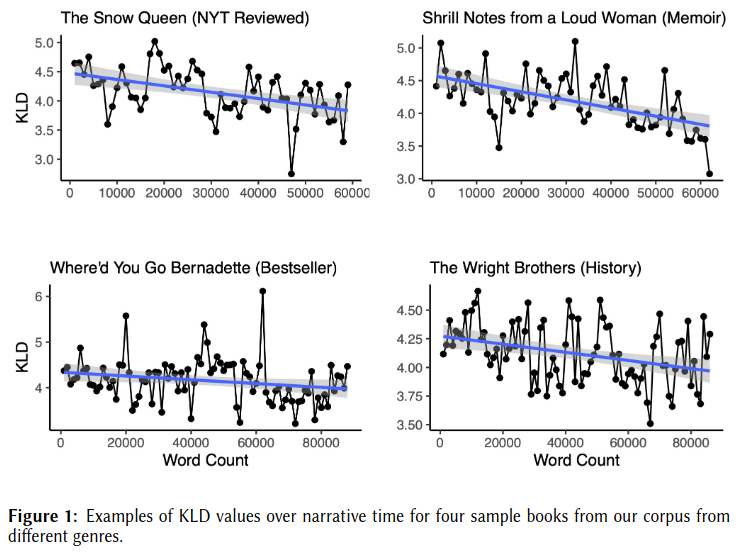
\includegraphics[width=.60\linewidth]{intro-to-ch/images/entrop_examples.png}
\end{frame}

\begin{frame}{Three hypothesis}
    \small
    \begin{itemize}
        \item<1-> \textbf{H1. Average Rate of Revelation}. \only<1>{We expect average revelation at the book level to vary by all of our measured social categories. Specifically, prior work [29] has indicated that fictional narratives are more predictable at the sentence level and thus we expect to see lower levels of average revelation with respect to fictionality at the document level. We also \textbf{expect average revelation to be negatively associated with reading level and positively associated with prestige} (more information being more “difficult” for readers to process and thus potentially more valued by elite readerships).}%
        \item<2-> \textbf{H2. The Slope of Revelation}. \only<2>{We expect there to be an \textbf{association between revelation and narrative time}. Prior theoretical work has suggested that narratives exhibit structural patterns [17], which has been confirmed in different ways through empirical work [5, 27, 11]. A general linear increase in surprise would support a theory of narrative investment in the value of plot twists (or “surprise endings”), while a general linear decrease would support the theory of narrative immersion, i.e. once novel information is introduced a narrative spends less time introducing more information (exploration) and more time exploiting known information. \textbf{While we expect there to be an association between revelation and time, prior work does not give clear indications of which directionality to expect}.}%
        \item<3->\textbf{H3. Dependency Patterns of Revelation}. \only<3>{Given assumptions about the value of narrative structure to narrative meaning, \textbf{we expect there to be discernible dependency patterns to the rise and fall of revelatio}n, with the present extent of revelation driven by that of the past in non-trivial ways (e.g., lagged dependency). While no prior work has suggested that narrative revelation should follow predictable dependency patterns, it could be the case that this is a latent structural feature to narrative plotting and potentially drives reader enjoyment.}
    \end{itemize}
\end{frame}

\subsection{Results}

\begin{frame}{Average Revelation Hypothesis (H1)}
    \begin{itemize}
        \item Compute the average value of $KLD_{T}$ over times T, with standardization according to book length in CONLIT data.
        \item Compute Cohen's : $d = \frac{\overline{DKL_{t_{1}}} - \overline{DKL_{t_{2}}}}{\sigma_{T}}$ where $t_{1}$ is one sample and $t_{2}$ another from $T$
        \item \textbf{Results:}
        \begin{itemize}
            \item Non fiction has higher average information revalation over time.
            \item Prestige has the inverse effect, and is twice most impactful as Age Level: contemporaneous prestigious books have lower entropy (lower amount of new information) from one spot to another on average.
        \end{itemize}
    \end{itemize}
\end{frame}

\begin{frame}{The Slope of Revelation (H2)}
    \begin{columns}
        \begin{column}{.7\textwidth}
            
            \begin{itemize}
                \item Regression analysis: find a function that would fit the curve.
                \item Correlates with H1: less and less revelations over time in general
                \item At local minima: the end of books have in general higher KLD (and so new information)
                \item ``We found that youth fiction was similarly associated with greater decreases of revelation over narrative time, but that prestige and point-of-view were not''
            \end{itemize}
        \end{column}
        \begin{column}{.3\textwidth}
            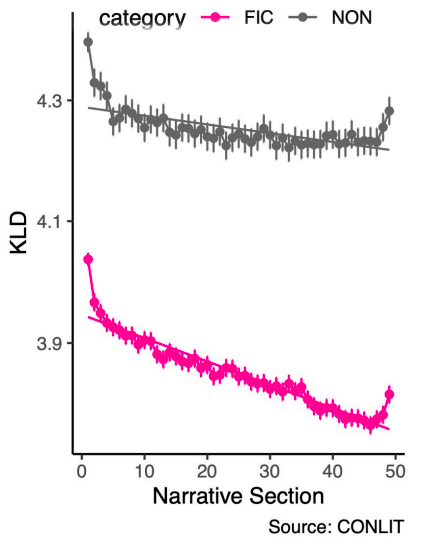
\includegraphics[width=\linewidth]{images/entropy_linear.png}
        \end{column}
    \end{columns}
\end{frame}

\begin{frame}{Dependency Patterns of Revelation (H3)}
    \begin{itemize}
        \item No clear period frequency regarding KLD.
        \item Use of ARIMA models (AutoRegressive, Integrated and Moving Average) who tries to identify the lag $p$ such that $KDL_{T}$ can be predicted by $KDL_{T-p}$ and a trend of order $d$, such that each $KDL_{T_{i}}$ fits a slop of its polynomial order.
        \item For our second variable, 39\% of all books exhibited autoregressive behavior ($d > 0$), meaning that in a strong minority of books the successive values of narrative revelation are correlated.
    \end{itemize}
\end{frame}


\subsection{Discussion}

\begin{frame}{A convincing article}
    \begin{itemize}
        \item The article is sound, well written and builds on previous knowledge, with a strong state-of-the-art \textit{à la} computer science / natural language processing.
        \item It provides not only a new method, but new results. 
        \item Code is not provided, reproducibility is lessened, but the overall explanations should make up for it.
    \end{itemize}
\end{frame}

\begin{frame}{With limitations ?}
    \begin{itemize}
        \item The use of word frequencies, as duly noted by the author, and word-to-word comparison lower the impact of the comparison: if I have $X_{T} = \text{I, eat, chocolate}$ and $X_{T-1} = \text{I, buy, kinders}$, is the information revelation that important ? The usage of embeddings to compare words, in one way or another, and map $X$ onto a semantic space with connected frequencies might allow for more fine grained results (see \cite{eder2022boostingwordfrequenciesauthorship}\footfullcite{eder2022boostingwordfrequenciesauthorship}).
        \item A smaller focus, on genres would have been interesting, beyond fictional/non fictional
    \end{itemize}
\end{frame}

\section{\textit{Operationalizing and Measuring Conflict in German Novels}, Haüssler et Gius, 2023}

\subsection{Summary}

\begin{frame}{Paper}
    \fullcite{operationalizing}
\end{frame}

\subsection{Results}

\subsection{Discussion}

\end{document}